\documentclass{beamer}
\usepackage[latin1]{inputenc}
%\usetheme{Montpellier}
\usetheme{Boadilla}
\usepackage{color, colortbl}
%\usecolortheme[RGB={204,51,255}]{structure}
%\usecolortheme[named=plum]{structure}
\usecolortheme[RGB={62,128,62}]{structure}
%\definecolor{dark}{rgb}{0.3,0.15,0.3}
%\definecolor{light}{rgb}{0.8,0.6,0.8}
\definecolor{reddish}{rgb}{.5,0.15,0.15}
\definecolor{dark}{rgb}{0.4,0.2,0.4}
\definecolor{darkgreen}{rgb}{0.25,0.5,0.25}
\definecolor{darkred}{rgb}{0.75,0.25,0.25}
\definecolor{darkblue}{rgb}{0.25,0.25,0.75}
\definecolor{light}{rgb}{0.8,0.6,0.8}
\definecolor{darklight}{rgb}{0.6,0.45,0.6}
\definecolor{newlight}{rgb}{0.6,0.8,0.8}
\definecolor{newdarklight}{rgb}{0.45,0.6,0.6}
\definecolor{reddish}{rgb}{.7,0.25,0.25}
\usepackage{graphicx}
\usepackage{pstricks}

\newcommand{\vi}{\color{blue}v_i\color{black}}
\newcommand{\hj}{\color{red}h_j\color{black}}
\newcommand{\hi}{\color{red}h_i\color{black}}

\newcommand{\vbf}{\color{blue}\mathbf{v}\color{black}}
\newcommand{\hbf}{\color{red}\mathbf{h}\color{black}}

\newcommand{\bigv}{\color{blue}V\color{black}}

\newcommand{\cor}{\color{reddish}{}}
\newcommand{\cob}{\color{black}{}}


\usepackage{tikz}
\usepackage{epstopdf}
\usetikzlibrary{positioning}
\newcommand*\eiadfamily{\fontencoding{OT1}\fontfamily{eiad}\selectfont}
\usepackage[OT1]{fontenc}

\title[How deep is deep]{How deep is deep enough? - Optimizing deep neural network architecture: Schilling et al}
\author{Conor Houghton}
\institute{deep reading journal club: 1811.01753}
\date{2019-10-17}

\begin{document}

\maketitle

\begin{frame}{Restricted Boltzmann Machines}

\def\layersep{2.5cm}

\begin{columns}
\begin{column}{0.5\textwidth}
$$
  E= - \sum \vi w_{ij}\hj
$$
  \color{reddish}
  \begin{flushleft}
which corresponds to the Hopfield-style dynamics:
\end{flushleft}
\color{black}

$$
  \vi=\left\{\begin{array}{cc}1&\sum_j w_{ij}\hj>0\\0&\mbox{otherwise}\end{array}\right.
  $$
\end{column}
\begin{column}{0.5\textwidth}
    \begin{center}  
\begin{tikzpicture}[shorten >=1pt,<->,draw=black!50, node distance=\layersep]
    \tikzstyle{every pin edge}=[<-,shorten <=1pt]
    \tikzstyle{neuron}=[circle,fill=black!25,minimum size=12pt,inner sep=0pt]
    \tikzstyle{input neuron}=[neuron, fill=blue!50];
    \tikzstyle{hidden neuron}=[neuron, fill=red!50];
    \tikzstyle{annot} = [text width=4em, text centered]

    % Draw the input layer nodes
    \foreach \name / \y in {1,...,5}
    % This is the same as writing \foreach \name / \y in {1/1,2/2,3/3,4/4}
    \node[input neuron] (I-\name) at (0,-\y cm) {};

    % Draw the hidden layer nodes
    \foreach \name / \y in {2,...,4}
   \node[hidden neuron] (H-\name) at (\layersep,-\y cm) {};

    % Connect every node in the input layer with every node in the
    % hidden layer.
    \foreach \source in {1,...,5}
        \foreach \dest in {2,...,4}
            \path (I-\source) edge (H-\dest);

    % Annotate the layers
    \node[annot,above of=I-1, node distance=1cm] (vl) {Visual layer};
    \node[annot,right of=vl] {Hidden layer};
\end{tikzpicture}

    \end{center}
\end{column}
\end{columns}

\end{frame}


\begin{frame}{Restricted Boltzmann Machines - Boltzmannitude}

\def\layersep{2.5cm}

\begin{columns}
\begin{column}{0.5\textwidth}
  \color{reddish}
  \begin{flushleft}
Imagine the network immersed in a heat bath so
\end{flushleft}
\color{black}
$$
P(\vbf,\hbf)=\frac{e^{-E(\vbf,\hbf)}}{Z}
$$
\color{reddish}

where \color{black}$Z$\color{reddish}{} is the partition function\color{black}
  $$
Z=\sum_{\vbf,\hbf}e^{-E(\vbf,\hbf)}
$$
\end{column}
\begin{column}{0.5\textwidth}
\begin{center}  
\begin{tikzpicture}[shorten >=1pt,<->,draw=black!50, node distance=\layersep]
    \tikzstyle{every pin edge}=[<-,shorten <=1pt]
    \tikzstyle{neuron}=[circle,fill=black!25,minimum size=12pt,inner sep=0pt]
    \tikzstyle{input neuron}=[neuron, fill=blue!50];
    \tikzstyle{hidden neuron}=[neuron, fill=red!50];
    \tikzstyle{annot} = [text width=4em, text centered]

    % Draw the input layer nodes
    \foreach \name / \y in {1,...,5}
    % This is the same as writing \foreach \name / \y in {1/1,2/2,3/3,4/4}
    \node[input neuron] (I-\name) at (0,-\y cm) {};

    % Draw the hidden layer nodes
    \foreach \name / \y in {2,...,4}
   \node[hidden neuron] (H-\name) at (\layersep,-\y cm) {};

    % Connect every node in the input layer with every node in the
    % hidden layer.
    \foreach \source in {1,...,5}
        \foreach \dest in {2,...,4}
            \path (I-\source) edge (H-\dest);

    % Annotate the layers
    \node[annot,above of=I-1, node distance=1cm] (vl) {Visual layer};
    \node[annot,right of=vl] {Hidden layer};
\end{tikzpicture}

\end{center}
\end{column}
\end{columns}

\end{frame}


\begin{frame}{Restricted Boltzmann Machines - Restrictiness}

\def\layersep{2.5cm}

\begin{columns}
\begin{column}{0.5\textwidth}
  \color{reddish}
  \begin{flushleft}
Since the machine is bipartite the nodes are conditionally independent
\end{flushleft}
\color{black}
\begin{eqnarray*}
  P(\vbf|\hbf)=\prod_{i}P(\vi|\hbf)\cr
  P(\hbf|\vbf)=\prod_{i}P(\hi|\vbf)\cr
\end{eqnarray*}
\end{column}
\begin{column}{0.5\textwidth}
\begin{center}  
\begin{tikzpicture}[shorten >=1pt,<->,draw=black!25, node distance=\layersep]
    \tikzstyle{every pin edge}=[<-,shorten <=1pt]
    \tikzstyle{neuron}=[circle,fill=black!25,minimum size=12pt,inner sep=0pt]
    \tikzstyle{input neuron}=[neuron, fill=blue!50];
    \tikzstyle{hidden neuron}=[neuron, fill=red!50];
    \tikzstyle{annot} = [text width=4em, text centered]

    % Draw the input layer nodes
    \foreach \name / \y in {1,...,5}
    % This is the same as writing \foreach \name / \y in {1/1,2/2,3/3,4/4}
    \node[input neuron] (I-\name) at (0,-\y cm) {};

    % Draw the hidden layer nodes
    \foreach \name / \y in {2,...,4}
   \node[hidden neuron] (H-\name) at (\layersep,-\y cm) {};

    % Connect every node in the input layer with every node in the
    % hidden layer.
    \foreach \source in {1,...,5}
        \foreach \dest in {2,...,4}
        \path (I-\source) edge (H-\dest);

    % Connect node 2 in the input layer with every node in the
    % hidden layer in black
    \foreach \dest in {2,...,4}
        \path (I-2) edge[black] (H-\dest);
        

    % Annotate the layers
    \node[annot,above of=I-1, node distance=1cm] (vl) {Visual layer};
    \node[annot,right of=vl] {Hidden layer};
\end{tikzpicture}

\end{center}
\end{column}
\end{columns}

\end{frame}


\begin{frame}{Restricted Boltzmann Machines - Restrictiness}

\def\layersep{2.5cm}

\begin{columns}
\begin{column}{0.5\textwidth}
  \color{reddish}
  \begin{flushleft}
Since the machine is bipartite the nodes are conditionally independent
\end{flushleft}
\color{black}
\begin{eqnarray*}
  P(\vbf|\hbf)=\prod_{i}P(\vi|\hbf)\cr
  P(\hbf|\vbf)=\prod_{i}P(\hi|\vbf)\cr
\end{eqnarray*}
\end{column}
\begin{column}{0.5\textwidth}
\begin{center}  
\begin{tikzpicture}[shorten >=1pt,<->,draw=black!25, node distance=\layersep]
    \tikzstyle{every pin edge}=[<-,shorten <=1pt]
    \tikzstyle{neuron}=[circle,fill=black!25,minimum size=12pt,inner sep=0pt]
    \tikzstyle{input neuron}=[neuron, fill=blue!50];
    \tikzstyle{hidden neuron}=[neuron, fill=red!50];
    \tikzstyle{annot} = [text width=4em, text centered]

    % Draw the input layer nodes
    \foreach \name / \y in {1,...,5}
    % This is the same as writing \foreach \name / \y in {1/1,2/2,3/3,4/4}
    \node[input neuron] (I-\name) at (0,-\y cm) {};

    % Draw the hidden layer nodes
    \foreach \name / \y in {2,...,4}
   \node[hidden neuron] (H-\name) at (\layersep,-\y cm) {};

    % Connect every node in the input layer with every node in the
    % hidden layer.
    \foreach \source in {1,...,5}
        \foreach \dest in {2,...,4}
        \path (I-\source) edge (H-\dest);

    % Connect every node in the input layer with node 3 in the
    % hidden layer in black
    \foreach \source in {1,...,5}
        \path (I-\source) edge[black] (H-3);
        
    % Annotate the layers
    \node[annot,above of=I-1, node distance=1cm] (vl) {Visual layer};
    \node[annot,right of=vl] {Hidden layer};
\end{tikzpicture}

\end{center}
\end{column}
\end{columns}

\end{frame}


\begin{frame}{Restricted Boltzmann Machines - Conditional Probability}

$$
  P(\vbf|\hbf)=\frac{1}{Z_{\hbf} } e^{-E(\vbf,\hbf)}
$$
  \color{reddish}where\color{black}{}
$$
  Z_{\hbf}=P(\hbf)=\sum_{\vbf} P(\vbf,\hbf)
  $$
\end{frame}

\begin{frame}{Restricted Boltzmann Machines - Conditional Probability}
\color{reddish}Now\color{black}
$$
e^{-E(\vbf,\hbf)}=\prod_ie^{\sum_j\vi w_{ij} \hj}
$$
\color{reddish}and\color{black}{}
$$
Z_{\hbf}= \prod_i\sum_{\vi=0,1}e^{\sum_j\vi w_{ij} \hj}
$$
\color{reddish}so\color{black}
$$
  P(\vbf|\hbf)=\prod_i \frac{e^{\sum_j\vi w_{ij} \hj}}{1+e^{\sum_jw_{ij} \hj}}
$$
\color{reddish}or, for example\color{black}
$$
  P(v_i=1|\hbf)=\sigma(\sum_jw_{ij}\hj)
$$
\color{reddish}where\color{black}{} $\sigma$\color{reddish}{} is the logistic function.\color{black}
\end{frame}



\begin{frame}{Restricted Boltzmann Machines - So?}
\color{reddish}Again\color{black}
$$
  P(\vi=1|\hbf)=\sigma(\sum_jw_{ij}\hj)
$$
\color{reddish}and\color{black}{}
$$
  P(\hi=1|\vbf)=\sigma(\sum_i \vi w_{ij})
$$
  \color{reddish}so we can easily sample from the layer.
  \begin{itemize}
    \item \cor{} The idea is to fix the $w_{ij}$ so that the $\vbf$\cor{} match a training set; the $\hbf$\cor{} then summarizes the input. 
\end{itemize}
\end{frame}



\begin{frame}{Restricted Boltzmann Machines - Example - input}
\color{reddish}The famous application of RBMs was on the Netflix data:\color{black}

\def\layersep{2.5cm}
\begin{center}
\begin{tikzpicture}[shorten >=1pt,->,draw=black!50, node distance=\layersep]
    \tikzstyle{every pin edge}=[<-,shorten <=1pt]
    \tikzstyle{neuron}=[circle,fill=black!25,minimum size=12pt,inner sep=0pt]
    \tikzstyle{input neuron}=[neuron, fill=blue!50];
    \tikzstyle{hidden neuron}=[neuron, fill=red!50];
    \tikzstyle{annot} = [text width=4em, text centered]
    
    \node[input neuron,fill=white,draw=black] (I1) at (0,-1cm) {};
    \node[input neuron,fill=blue!50,draw=black] (I2) at (0,-2cm) {};
    \node[input neuron,fill=white,draw=black] (I3) at (0,-3cm) {};
    \node[input neuron,fill=blue!50,draw=black] (I4) at (0,-4cm) {};
    \node[input neuron,fill=black!25,draw=black] (I5) at (0,-5cm) {};
    
    \node[hidden neuron,fill=red!20,draw=black] (H2) at (\layersep,-2cm) {};
    \node[hidden neuron,fill=red!10,draw=black] (H3) at (\layersep,-3cm) {};
    \node[hidden neuron,fill=red!75,draw=black] (H4) at (\layersep,-4cm) {};

    \node[left of =I1] (mI-1){His Girl Friday};
    \node[left of =I2] (mI-2){Goodfellas};
    \node[left of =I3] (mI-3){\`A Bout de Souffle};
    \node[left of =I4] (mI-4){The Godfather II};
    \node[left of =I5] (mI-4){Scarface};

    \node[right of =H2](gH-1){Classic};
    \node[right of =H3](gH-2){New Wave};
    \node[right of =H4](gH-3){US Gangster};

    % Connect every node in the input layer with every node in the
    % hidden layer.
    \foreach \source in {1,...,4}
        \foreach \dest in {2,...,4}
            \path (I-\source) edge (H-\dest);

    % Annotate the layers
    \node[annot,above of=I1, node distance=1cm] (vl) {Visual layer};
    \node[annot,right of=vl] {Hidden layer};
\end{tikzpicture}
\end{center}
\end{frame}

\begin{frame}{Restricted Boltzmann Machines - Example - output}
\color{reddish}The famous application of RBMs was on the Netflix data:\color{black}

\def\layersep{2.5cm}
\begin{center}
\begin{tikzpicture}[shorten >=1pt,<-,draw=black!50, node distance=\layersep]
    \tikzstyle{every pin edge}=[<-,shorten <=1pt]
    \tikzstyle{neuron}=[circle,fill=black!25,minimum size=12pt,inner sep=0pt]
    \tikzstyle{input neuron}=[neuron, fill=blue!50];
    \tikzstyle{hidden neuron}=[neuron, fill=red!50];
    \tikzstyle{annot} = [text width=4em, text centered]
    
    \node[input neuron,fill=blue!05,draw=black] (I1) at (0,-1cm) {};
    \node[input neuron,fill=blue!50,draw=black] (I2) at (0,-2cm) {};
    \node[input neuron,fill=blue!10,draw=black] (I3) at (0,-3cm) {};
    \node[input neuron,fill=blue!40,draw=black] (I4) at (0,-4cm) {};
    \node[input neuron,fill=blue!50,draw=black] (I5) at (0,-5cm) {};
    
    \node[hidden neuron,fill=red!20,draw=black] (H2) at (\layersep,-2cm) {};
    \node[hidden neuron,fill=red!10,draw=black] (H3) at (\layersep,-3cm) {};
    \node[hidden neuron,fill=red!75,draw=black] (H4) at (\layersep,-4cm) {};

    \node[left of =I1] (mI-1){His Girl Friday};
    \node[left of =I2] (mI-2){Goodfellas};
    \node[left of =I3] (mI-3){\`A Bout de Souffle};
    \node[left of =I4] (mI-4){The Godfather II};
    \node[left of =I5] (mI-4){Scarface};

    \node[right of =H2](gH-1){Classic};
    \node[right of =H3](gH-2){New Wave};
    \node[right of =H4](gH-3){US Gangster};

    % Connect every node in the input layer with every node in the
    % hidden layer.
    \foreach \source in {1,...,5}
        \foreach \dest in {2,...,4}
            \path (I-\source) edge (H-\dest);

    % Annotate the layers
    \node[annot,above of=I1, node distance=1cm] (vl) {Visual layer};
    \node[annot,right of=vl] {Hidden layer};
\end{tikzpicture}
\end{center}

\end{frame}

\begin{frame}{Restricted Boltzmann Machines - Training}

  \cor{}The goal is to maximize\cob{} $P(\vbf)$\cor{} for \cob{}$\vbf\in \color{blue}V\color{black}$\cor{}, a training set:\cob{}
  $$
    W=\mbox{arg}\,\mbox{max}\left\langle P(\vbf)\right\rangle_{\bigv}=\mbox{arg}\,\mbox{max}\left\langle\log{P(\vbf)}\right\rangle_{\bigv}
  $$
    \cor{}Now for convenience lets write\cob{}
    $$
    f(\vbf,\hbf;W)=e^{\sum_{ij}\vi w_{ij} \hi}
    $$
\cor{}so\cob{}
  $$
  \log{P(\vbf)}=-\log{Z}+\log{f(\vbf,\hbf)}
  $$
  \cor{}and so we are trying to minimize\cob{}
  $$
  \mathcal{E}=\log{Z}-\left\langle \log{f(\vbf,\hbf)} \right\rangle_{\bigv}
  $$
  \end{frame}
  

\begin{frame}{Restricted Boltzmann Machines - Training}

  \cor{}Now\cob{}
  $$
  \frac{d\log{Z}}{dw_{ij}}=\frac{1}{Z}\sum_{\vbf}\frac{d f(\vbf,\hbf)}{dw_{ij}}= \sum_{\vbf}\frac{f(\vbf,\hbf)}{Z}\frac{d \log{f(\vbf,\hbf)}}{dw_{ij}} 
  $$
  \cor{}Hence\cob{}
  $$
  \frac{d\log{Z}}{dw_{ij}}=\left\langle\frac{d \log{f(\vbf,\hbf)}}{dw_{ij}}\right\rangle_{\vbf} 
  $$
  \cor{}This gives\cob{}
  $$
  \frac{d\mathcal{E}}{dw_{ij}}=\left\langle\frac{d \log{f(\vbf,\hbf)}}{dw_{ij}}\right\rangle_{\vbf} -\left\langle\frac{d \log{f(\vbf,\hbf)}}{dw_{ij}}\right\rangle_{\bigv}
  $$
  \end{frame}


\begin{frame}{Restricted Boltzmann Machines - Contrastive divergence}

  $$
  \mathcal{E}=\color{green}\left\langle\color{black}\frac{d \log{f(\vbf,\hbf)}}{dw_{ij}}\color{green}\right\rangle_{\vbf}\color{black}{} -\color{orange}\left\langle\color{black}\frac{d \log{f(\vbf,\hbf)}}{dw_{ij}}\color{orange}\right\rangle\color{black}_{\vbf\in\bigv}
  $$
  
  \cor{}Now we can work this out by sampling:
  $$
  \color{blue}\mathbf{v}_1\color{black}\rightarrow\color{red}\mathbf{h}_1\color{black}\rightarrow
  \color{blue}\mathbf{v}_2\color{black}\rightarrow\color{red}\mathbf{h}_2\color{black}\rightarrow
  \color{blue}\mathbf{v}_3\color{black}\rightarrow\color{red}\mathbf{h}_4\color{black}\rightarrow
  \color{blue}\mathbf{v}_5\color{black}\rightarrow\color{red}\mathbf{h}_5\color{black}\rightarrow
  \color{blue}\mathbf{v}_6\color{black}\rightarrow\color{red}\mathbf{h}_6\color{black}\rightarrow\ldots
  $$
\cor{}with\cob{} $\color{blue}\mathbf{v}_1\color{black}=\vbf$\cob{}
  $$
  \color{orange}\boxed{\color{blue}\mathbf{v}_1\color{black}\rightarrow
  \color{red}\mathbf{h}_1\color{black}}\color{black}\rightarrow\color{blue}\mathbf{v}_2\color{black}
  \rightarrow\color{red}\mathbf{h}_2\color{black}\rightarrow
  \color{blue}\mathbf{v}_3\color{black}\rightarrow\color{red}\mathbf{h}_4\color{black}\rightarrow
  \color{green}\boxed{\color{blue}\mathbf{v}_5\color{black}\rightarrow\color{red}\mathbf{h}_5\color{black}}\color{black}\rightarrow
  \color{blue}\mathbf{v}_6\color{black}\rightarrow\color{red}\mathbf{h}_6\color{black}\rightarrow\ldots
 $$
\cor{}and Hinton's contrastive divergence says you can get away with  
  $$
  \color{orange}\boxed{\color{blue}\mathbf{v}_1\color{black}\rightarrow
  \color{red}\mathbf{h}_1\color{black}}\color{black}\rightarrow \color{green}\boxed{\color{blue}\mathbf{v}_2\color{black}
  \rightarrow\color{red}\mathbf{h}_2\color{black}}\color{black}\rightarrow
  \color{blue}\mathbf{v}_3\color{black}\rightarrow\color{red}\mathbf{h}_4\color{black}\rightarrow
  \color{blue}\mathbf{v}_5\color{black}\rightarrow\color{red}\mathbf{h}_5\color{black}\rightarrow
  \color{blue}\mathbf{v}_6\color{black}\rightarrow\color{red}\mathbf{h}_6\color{black}\rightarrow\ldots
  $$

  \end{frame}

\begin{frame}{Restricted Boltzmann Machines - Contrastive divergence}

  \cor{} In fact, the derivative are very straightforward since\cob{}
  $$
  \log{f(\vbf,\hbf;W)}={\sum_{ij}\vi w_{ij} \hi}
  $$
  \cor{} so the gradient is just given by outer products\cob{}
  $$
  \delta w_{ij}\propto \vi \hj-\color{blue}v_i'\color{red}h_j'\color{black}
  $$
  \cor{}where\cob{}
  $$
  \color{blue}\mathbf{v}\color{black}\rightarrow\color{red}\mathbf{h}\color{black}\rightarrow
  \color{blue}\mathbf{v}'\color{black}\rightarrow\color{red}\mathbf{h}'\color{black}\rightarrow
  \ldots
  $$
\end{frame}
  
\begin{frame}{Deep Belief Network}
\def\layersep{2.5cm}
  \begin{center}
    \begin{tikzpicture}[shorten >=1pt,<->,draw=black!50, node distance=\layersep]
    \tikzstyle{every pin edge}=[<-,shorten <=1pt]
    \tikzstyle{neuron}=[circle,fill=black!25,minimum size=12pt,inner sep=0pt]
    \tikzstyle{input neuron}=[neuron, fill=blue!50];
    \tikzstyle{hidden neuron}=[neuron, fill=red!50];
    \tikzstyle{dark neuron}=[neuron, fill=black!50];
    \tikzstyle{annot} = [text width=4em, text centered]

    % Draw the input layer nodes
    \foreach \name / \y in {1,...,5}
    % This is the same as writing \foreach \name / \y in {1/1,2/2,3/3,4/4}
    \node[input neuron] (I-\name) at (0,-\y cm) {};

    % Draw the hidden 1 layer nodes
    \foreach \name / \y in {2,...,4}
   \node[hidden neuron] (H1-\name) at (\layersep,-\y cm) {};


    % Draw the hidden 2 layer nodes
   \foreach \name / \y in {2,...,4}
   \node[hidden neuron] (H2-\name) at (2*\layersep,-\y cm) {};

   
    % Draw the hidden 3 layer nodes
   \foreach \name / \y in {2,...,4}
   \node[hidden neuron] (H3-\name) at (3*\layersep,-\y cm) {};

   
    % Draw the hidden 4 layer nodes
   \foreach \name / \y in {2,...,4}
   \node[hidden neuron] (H4-\name) at (4*\layersep,-\y cm) {};


   
    % Connect every node in the input layer with every node in the
    % hidden layer.
    \foreach \source in {1,...,5}
        \foreach \dest in {2,...,4}
            \path (I-\source) edge (H1-\dest);


    \foreach \source in {2,...,4}
        \foreach \dest in {2,...,4}
            \path (H1-\source) edge (H2-\dest);


    \foreach \source in {2,...,4}
        \foreach \dest in {2,...,4}
            \path (H2-\source) edge (H3-\dest);


    \foreach \source in {2,...,4}
        \foreach \dest in {2,...,4}
            \path (H3-\source) edge (H4-\dest);
            
    % Annotate the layers
    \node[annot,above of=I-1, node distance=1cm] (vl) {Visual layer};
    \node[annot,right of=vl](h1l) {Hidden layer 1};
    \node[annot,right of=h1l](h2l) {Hidden layer 2};
    \node[annot,right of=h2l](h3l) {Hidden layer 3};
    \node[annot,right of=h3l](h4l) {Hidden layer 4};
    
\end{tikzpicture}

  \end{center}
\end{frame}

\begin{frame}{Deep Belief Network - learning}
\def\layersep{2.5cm}
  \begin{center}
    \begin{tikzpicture}[shorten >=1pt,<->,draw=black!10, node distance=\layersep]
    \tikzstyle{every pin edge}=[<-,shorten <=1pt]
    \tikzstyle{neuron}=[circle,fill=black!25,minimum size=12pt,inner sep=0pt]
    \tikzstyle{input neuron}=[neuron, fill=blue!50];
    \tikzstyle{hidden neuron}=[neuron, fill=red!50];
    \tikzstyle{dark neuron}=[neuron, fill=black!50];
    \tikzstyle{annot} = [text width=4em, text centered]

    % Draw the input layer nodes
    \foreach \name / \y in {1,...,5}
    % This is the same as writing \foreach \name / \y in {1/1,2/2,3/3,4/4}
    \node[input neuron] (I-\name) at (0,-\y cm) {};

    % Draw the hidden 1 layer nodes
    \foreach \name / \y in {2,...,4}
   \node[hidden neuron] (H1-\name) at (\layersep,-\y cm) {};

    % Draw the hidden 2 layer nodes
   \foreach \name / \y in {2,...,4}
   \node[dark neuron] (H2-\name) at (2*\layersep,-\y cm) {};

   
    % Draw the hidden 3 layer nodes
   \foreach \name / \y in {2,...,4}
   \node[dark neuron] (H3-\name) at (3*\layersep,-\y cm) {};

   
    % Draw the hidden 4 layer nodes
   \foreach \name / \y in {2,...,4}
   \node[dark neuron] (H4-\name) at (4*\layersep,-\y cm) {};
   
    % Connect every node in the input layer with every node in the
    % hidden layer.
    \foreach \source in {1,...,5}
        \foreach \dest in {2,...,4}
            \path (I-\source) edge (H1-\dest);


    \foreach \source in {2,...,4}
        \foreach \dest in {2,...,4}
            \path (H1-\source) edge (H2-\dest);


    \foreach \source in {2,...,4}
        \foreach \dest in {2,...,4}
            \path (H2-\source) edge (H3-\dest);


    \foreach \source in {2,...,4}
        \foreach \dest in {2,...,4}
            \path (H3-\source) edge (H4-\dest);
            
    % Annotate the layers
    \node[annot,above of=I-1, node distance=1cm] (vl) {Visual layer};
    \node[annot,right of=vl](h1l) {Hidden layer 1};
    \node[annot,right of=h1l](h2l) {Hidden layer 2};
    \node[annot,right of=h2l](h3l) {Hidden layer 3};
    \node[annot,right of=h3l](h4l) {Hidden layer 4};
    
\end{tikzpicture}

  \end{center}
\end{frame}

\begin{frame}{Deep Belief Network - learning}
\def\layersep{2.5cm}
  \begin{center}
    \begin{tikzpicture}[shorten >=1pt,<->,draw=black!10, node distance=\layersep]
    \tikzstyle{every pin edge}=[<-,shorten <=1pt]
    \tikzstyle{neuron}=[circle,fill=black!25,minimum size=12pt,inner sep=0pt]
    \tikzstyle{input neuron}=[neuron, fill=blue!50];
    \tikzstyle{hidden neuron}=[neuron, fill=red!50];
    \tikzstyle{dark neuron}=[neuron, fill=black!50];
    \tikzstyle{annot} = [text width=4em, text centered]

    % Draw the input layer nodes
    \foreach \name / \y in {1,...,5}
    % This is the same as writing \foreach \name / \y in {1/1,2/2,3/3,4/4}
    \node[input neuron] (I-\name) at (0,-\y cm) {};

    % Draw the hidden 1 layer nodes
    \foreach \name / \y in {2,...,4}
   \node[hidden neuron] (H1-\name) at (\layersep,-\y cm) {};

    % Draw the hidden 2 layer nodes
   \foreach \name / \y in {2,...,4}
   \node[dark neuron] (H2-\name) at (2*\layersep,-\y cm) {};

   
    % Draw the hidden 3 layer nodes
   \foreach \name / \y in {2,...,4}
   \node[dark neuron] (H3-\name) at (3*\layersep,-\y cm) {};

   
    % Draw the hidden 4 layer nodes
   \foreach \name / \y in {2,...,4}
   \node[dark neuron] (H4-\name) at (4*\layersep,-\y cm) {};
   
    % Connect every node in the input layer with every node in the
    % hidden layer.
    \foreach \source in {1,...,5}
        \foreach \dest in {2,...,4}
            \path (I-\source) edge[draw=black!75] (H1-\dest);


    \foreach \source in {2,...,4}
        \foreach \dest in {2,...,4}
            \path (H1-\source) edge (H2-\dest);


    \foreach \source in {2,...,4}
        \foreach \dest in {2,...,4}
            \path (H2-\source) edge (H3-\dest);


    \foreach \source in {2,...,4}
        \foreach \dest in {2,...,4}
            \path (H3-\source) edge (H4-\dest);
            
    % Annotate the layers
    \node[annot,above of=I-1, node distance=1cm] (vl) {Visual layer};
    \node[annot,right of=vl](h1l) {Hidden layer 1};
    \node[annot,right of=h1l](h2l) {Hidden layer 2};
    \node[annot,right of=h2l](h3l) {Hidden layer 3};
    \node[annot,right of=h3l](h4l) {Hidden layer 4};
    
\end{tikzpicture}

  \end{center}
\end{frame}


\begin{frame}{Deep Belief Network - learning}
\def\layersep{2.5cm}
  \begin{center}
    \begin{tikzpicture}[shorten >=1pt,<->,draw=black!10, node distance=\layersep]
    \tikzstyle{every pin edge}=[<-,shorten <=1pt]
    \tikzstyle{neuron}=[circle,fill=black!25,minimum size=12pt,inner sep=0pt]
    \tikzstyle{input neuron}=[neuron, fill=blue!50];
    \tikzstyle{hidden neuron}=[neuron, fill=red!50];
    \tikzstyle{dark neuron}=[neuron, fill=black!50];
    \tikzstyle{annot} = [text width=4em, text centered]

    % Draw the input layer nodes
    \foreach \name / \y in {1,...,5}
    % This is the same as writing \foreach \name / \y in {1/1,2/2,3/3,4/4}
    \node[dark neuron] (I-\name) at (0,-\y cm) {};

    % Draw the hidden 1 layer nodes
    \foreach \name / \y in {2,...,4}
   \node[input neuron] (H1-\name) at (\layersep,-\y cm) {};

    % Draw the hidden 2 layer nodes
   \foreach \name / \y in {2,...,4}
   \node[hidden neuron] (H2-\name) at (2*\layersep,-\y cm) {};

   
    % Draw the hidden 3 layer nodes
   \foreach \name / \y in {2,...,4}
   \node[dark neuron] (H3-\name) at (3*\layersep,-\y cm) {};

   
    % Draw the hidden 4 layer nodes
   \foreach \name / \y in {2,...,4}
   \node[dark neuron] (H4-\name) at (4*\layersep,-\y cm) {};
   
    % Connect every node in the input layer with every node in the
    % hidden layer.
    \foreach \source in {1,...,5}
        \foreach \dest in {2,...,4}
            \path (I-\source) edge[draw=black!75] (H1-\dest);


    \foreach \source in {2,...,4}
        \foreach \dest in {2,...,4}
            \path (H1-\source) edge (H2-\dest);


    \foreach \source in {2,...,4}
        \foreach \dest in {2,...,4}
            \path (H2-\source) edge (H3-\dest);


    \foreach \source in {2,...,4}
        \foreach \dest in {2,...,4}
            \path (H3-\source) edge (H4-\dest);
            
    % Annotate the layers
    \node[annot,above of=I-1, node distance=1cm] (vl) {Visual layer};
    \node[annot,right of=vl](h1l) {Hidden layer 1};
    \node[annot,right of=h1l](h2l) {Hidden layer 2};
    \node[annot,right of=h2l](h3l) {Hidden layer 3};
    \node[annot,right of=h3l](h4l) {Hidden layer 4};
    
\end{tikzpicture}

  \end{center}
\end{frame}


\begin{frame}{Deep Belief Network - learning}
\def\layersep{2.5cm}
  \begin{center}
    \begin{tikzpicture}[shorten >=1pt,<->,draw=black!10, node distance=\layersep]
    \tikzstyle{every pin edge}=[<-,shorten <=1pt]
    \tikzstyle{neuron}=[circle,fill=black!25,minimum size=12pt,inner sep=0pt]
    \tikzstyle{input neuron}=[neuron, fill=blue!50];
    \tikzstyle{hidden neuron}=[neuron, fill=red!50];
    \tikzstyle{dark neuron}=[neuron, fill=black!50];
    \tikzstyle{annot} = [text width=4em, text centered]

    % Draw the input layer nodes
    \foreach \name / \y in {1,...,5}
    % This is the same as writing \foreach \name / \y in {1/1,2/2,3/3,4/4}
    \node[dark neuron] (I-\name) at (0,-\y cm) {};

    % Draw the hidden 1 layer nodes
    \foreach \name / \y in {2,...,4}
   \node[input neuron] (H1-\name) at (\layersep,-\y cm) {};

    % Draw the hidden 2 layer nodes
   \foreach \name / \y in {2,...,4}
   \node[hidden neuron] (H2-\name) at (2*\layersep,-\y cm) {};

   
    % Draw the hidden 3 layer nodes
   \foreach \name / \y in {2,...,4}
   \node[dark neuron] (H3-\name) at (3*\layersep,-\y cm) {};

   
    % Draw the hidden 4 layer nodes
   \foreach \name / \y in {2,...,4}
   \node[dark neuron] (H4-\name) at (4*\layersep,-\y cm) {};
   
    % Connect every node in the input layer with every node in the
    % hidden layer.
    \foreach \source in {1,...,5}
        \foreach \dest in {2,...,4}
            \path (I-\source) edge[draw=black!75] (H1-\dest);


    \foreach \source in {2,...,4}
        \foreach \dest in {2,...,4}
            \path (H1-\source) edge[draw=black!75] (H2-\dest);


    \foreach \source in {2,...,4}
        \foreach \dest in {2,...,4}
            \path (H2-\source) edge (H3-\dest);


    \foreach \source in {2,...,4}
        \foreach \dest in {2,...,4}
            \path (H3-\source) edge (H4-\dest);
            
    % Annotate the layers
    \node[annot,above of=I-1, node distance=1cm] (vl) {Visual layer};
    \node[annot,right of=vl](h1l) {Hidden layer 1};
    \node[annot,right of=h1l](h2l) {Hidden layer 2};
    \node[annot,right of=h2l](h3l) {Hidden layer 3};
    \node[annot,right of=h3l](h4l) {Hidden layer 4};
    
\end{tikzpicture}

  \end{center}
\end{frame}


\begin{frame}{Deep Belief Network - learning}
\def\layersep{2.5cm}
  \begin{center}
    \begin{tikzpicture}[shorten >=1pt,<->,draw=black!10, node distance=\layersep]
    \tikzstyle{every pin edge}=[<-,shorten <=1pt]
    \tikzstyle{neuron}=[circle,fill=black!25,minimum size=12pt,inner sep=0pt]
    \tikzstyle{input neuron}=[neuron, fill=blue!50];
    \tikzstyle{hidden neuron}=[neuron, fill=red!50];
    \tikzstyle{dark neuron}=[neuron, fill=black!50];
    \tikzstyle{annot} = [text width=4em, text centered]

    % Draw the input layer nodes
    \foreach \name / \y in {1,...,5}
    % This is the same as writing \foreach \name / \y in {1/1,2/2,3/3,4/4}
    \node[dark neuron] (I-\name) at (0,-\y cm) {};

    % Draw the hidden 1 layer nodes
    \foreach \name / \y in {2,...,4}
   \node[dark neuron] (H1-\name) at (\layersep,-\y cm) {};

    % Draw the hidden 2 layer nodes
   \foreach \name / \y in {2,...,4}
   \node[input neuron] (H2-\name) at (2*\layersep,-\y cm) {};

   
    % Draw the hidden 3 layer nodes
   \foreach \name / \y in {2,...,4}
   \node[hidden neuron] (H3-\name) at (3*\layersep,-\y cm) {};

   
    % Draw the hidden 4 layer nodes
   \foreach \name / \y in {2,...,4}
   \node[dark neuron] (H4-\name) at (4*\layersep,-\y cm) {};
   
    % Connect every node in the input layer with every node in the
    % hidden layer.
    \foreach \source in {1,...,5}
        \foreach \dest in {2,...,4}
            \path (I-\source) edge[draw=black!75] (H1-\dest);


    \foreach \source in {2,...,4}
        \foreach \dest in {2,...,4}
            \path (H1-\source) edge[draw=black!75] (H2-\dest);


    \foreach \source in {2,...,4}
        \foreach \dest in {2,...,4}
            \path (H2-\source) edge (H3-\dest);


    \foreach \source in {2,...,4}
        \foreach \dest in {2,...,4}
            \path (H3-\source) edge (H4-\dest);
            
    % Annotate the layers
    \node[annot,above of=I-1, node distance=1cm] (vl) {Visual layer};
    \node[annot,right of=vl](h1l) {Hidden layer 1};
    \node[annot,right of=h1l](h2l) {Hidden layer 2};
    \node[annot,right of=h2l](h3l) {Hidden layer 3};
    \node[annot,right of=h3l](h4l) {Hidden layer 4};
    
\end{tikzpicture}

  \end{center}
\end{frame}


\begin{frame}{Deep Belief Network - learning}
\def\layersep{2.5cm}
  \begin{center}
    \begin{tikzpicture}[shorten >=1pt,<->,draw=black!10, node distance=\layersep]
    \tikzstyle{every pin edge}=[<-,shorten <=1pt]
    \tikzstyle{neuron}=[circle,fill=black!25,minimum size=12pt,inner sep=0pt]
    \tikzstyle{input neuron}=[neuron, fill=blue!50];
    \tikzstyle{hidden neuron}=[neuron, fill=red!50];
    \tikzstyle{dark neuron}=[neuron, fill=black!50];
    \tikzstyle{annot} = [text width=4em, text centered]

    % Draw the input layer nodes
    \foreach \name / \y in {1,...,5}
    % This is the same as writing \foreach \name / \y in {1/1,2/2,3/3,4/4}
    \node[dark neuron] (I-\name) at (0,-\y cm) {};

    % Draw the hidden 1 layer nodes
    \foreach \name / \y in {2,...,4}
   \node[dark neuron] (H1-\name) at (\layersep,-\y cm) {};

    % Draw the hidden 2 layer nodes
   \foreach \name / \y in {2,...,4}
   \node[input neuron] (H2-\name) at (2*\layersep,-\y cm) {};

   
    % Draw the hidden 3 layer nodes
   \foreach \name / \y in {2,...,4}
   \node[hidden neuron] (H3-\name) at (3*\layersep,-\y cm) {};

   
    % Draw the hidden 4 layer nodes
   \foreach \name / \y in {2,...,4}
   \node[dark neuron] (H4-\name) at (4*\layersep,-\y cm) {};
   
    % Connect every node in the input layer with every node in the
    % hidden layer.
    \foreach \source in {1,...,5}
        \foreach \dest in {2,...,4}
            \path (I-\source) edge[draw=black!75] (H1-\dest);


    \foreach \source in {2,...,4}
        \foreach \dest in {2,...,4}
            \path (H1-\source) edge[draw=black!75] (H2-\dest);


    \foreach \source in {2,...,4}
        \foreach \dest in {2,...,4}
            \path (H2-\source) edge[draw=black!75] (H3-\dest);


    \foreach \source in {2,...,4}
        \foreach \dest in {2,...,4}
            \path (H3-\source) edge (H4-\dest);
            
    % Annotate the layers
    \node[annot,above of=I-1, node distance=1cm] (vl) {Visual layer};
    \node[annot,right of=vl](h1l) {Hidden layer 1};
    \node[annot,right of=h1l](h2l) {Hidden layer 2};
    \node[annot,right of=h2l](h3l) {Hidden layer 3};
    \node[annot,right of=h3l](h4l) {Hidden layer 4};
    
\end{tikzpicture}

  \end{center}
\end{frame}



\begin{frame}{Deep Belief Network - learning}
\def\layersep{2.5cm}
  \begin{center}
    \begin{tikzpicture}[shorten >=1pt,<->,draw=black!10, node distance=\layersep]
    \tikzstyle{every pin edge}=[<-,shorten <=1pt]
    \tikzstyle{neuron}=[circle,fill=black!25,minimum size=12pt,inner sep=0pt]
    \tikzstyle{input neuron}=[neuron, fill=blue!50];
    \tikzstyle{hidden neuron}=[neuron, fill=red!50];
    \tikzstyle{dark neuron}=[neuron, fill=black!50];
    \tikzstyle{annot} = [text width=4em, text centered]

    % Draw the input layer nodes
    \foreach \name / \y in {1,...,5}
    % This is the same as writing \foreach \name / \y in {1/1,2/2,3/3,4/4}
    \node[dark neuron] (I-\name) at (0,-\y cm) {};

    % Draw the hidden 1 layer nodes
    \foreach \name / \y in {2,...,4}
   \node[dark neuron] (H1-\name) at (\layersep,-\y cm) {};

    % Draw the hidden 2 layer nodes
   \foreach \name / \y in {2,...,4}
   \node[dark neuron] (H2-\name) at (2*\layersep,-\y cm) {};

   
    % Draw the hidden 3 layer nodes
   \foreach \name / \y in {2,...,4}
   \node[input neuron] (H3-\name) at (3*\layersep,-\y cm) {};

   
    % Draw the hidden 4 layer nodes
   \foreach \name / \y in {2,...,4}
   \node[hidden neuron] (H4-\name) at (4*\layersep,-\y cm) {};
   
    % Connect every node in the input layer with every node in the
    % hidden layer.
    \foreach \source in {1,...,5}
        \foreach \dest in {2,...,4}
            \path (I-\source) edge[draw=black!75] (H1-\dest);


    \foreach \source in {2,...,4}
        \foreach \dest in {2,...,4}
            \path (H1-\source) edge[draw=black!75] (H2-\dest);


    \foreach \source in {2,...,4}
        \foreach \dest in {2,...,4}
            \path (H2-\source) edge[draw=black!75] (H3-\dest);


    \foreach \source in {2,...,4}
        \foreach \dest in {2,...,4}
            \path (H3-\source) edge (H4-\dest);
            
    % Annotate the layers
    \node[annot,above of=I-1, node distance=1cm] (vl) {Visual layer};
    \node[annot,right of=vl](h1l) {Hidden layer 1};
    \node[annot,right of=h1l](h2l) {Hidden layer 2};
    \node[annot,right of=h2l](h3l) {Hidden layer 3};
    \node[annot,right of=h3l](h4l) {Hidden layer 4};
    
\end{tikzpicture}

  \end{center}
\end{frame}


\begin{frame}{Deep Belief Network - learning}
\def\layersep{2.5cm}
  \begin{center}
    \begin{tikzpicture}[shorten >=1pt,<->,draw=black!10, node distance=\layersep]
    \tikzstyle{every pin edge}=[<-,shorten <=1pt]
    \tikzstyle{neuron}=[circle,fill=black!25,minimum size=12pt,inner sep=0pt]
    \tikzstyle{input neuron}=[neuron, fill=blue!50];
    \tikzstyle{hidden neuron}=[neuron, fill=red!50];
    \tikzstyle{dark neuron}=[neuron, fill=black!50];
    \tikzstyle{annot} = [text width=4em, text centered]

    % Draw the input layer nodes
    \foreach \name / \y in {1,...,5}
    % This is the same as writing \foreach \name / \y in {1/1,2/2,3/3,4/4}
    \node[dark neuron] (I-\name) at (0,-\y cm) {};

    % Draw the hidden 1 layer nodes
    \foreach \name / \y in {2,...,4}
   \node[dark neuron] (H1-\name) at (\layersep,-\y cm) {};

    % Draw the hidden 2 layer nodes
   \foreach \name / \y in {2,...,4}
   \node[dark neuron] (H2-\name) at (2*\layersep,-\y cm) {};

   
    % Draw the hidden 3 layer nodes
   \foreach \name / \y in {2,...,4}
   \node[input neuron] (H3-\name) at (3*\layersep,-\y cm) {};

   
    % Draw the hidden 4 layer nodes
   \foreach \name / \y in {2,...,4}
   \node[hidden neuron] (H4-\name) at (4*\layersep,-\y cm) {};
   
    % Connect every node in the input layer with every node in the
    % hidden layer.
    \foreach \source in {1,...,5}
        \foreach \dest in {2,...,4}
            \path (I-\source) edge[draw=black!75] (H1-\dest);


    \foreach \source in {2,...,4}
        \foreach \dest in {2,...,4}
            \path (H1-\source) edge[draw=black!75] (H2-\dest);


    \foreach \source in {2,...,4}
        \foreach \dest in {2,...,4}
            \path (H2-\source) edge[draw=black!75] (H3-\dest);


    \foreach \source in {2,...,4}
        \foreach \dest in {2,...,4}
            \path (H3-\source) edge[draw=black!75] (H4-\dest);
            
    % Annotate the layers
    \node[annot,above of=I-1, node distance=1cm] (vl) {Visual layer};
    \node[annot,right of=vl](h1l) {Hidden layer 1};
    \node[annot,right of=h1l](h2l) {Hidden layer 2};
    \node[annot,right of=h2l](h3l) {Hidden layer 3};
    \node[annot,right of=h3l](h4l) {Hidden layer 4};
    
\end{tikzpicture}

  \end{center}
\end{frame}

  
\begin{frame}{Deep Belief Network - encoding}
\def\layersep{2.5cm}
  \begin{center}
    \begin{tikzpicture}[shorten >=1pt,<->,draw=black!50, node distance=\layersep]
    \tikzstyle{every pin edge}=[<-,shorten <=1pt]
    \tikzstyle{neuron}=[circle,fill=black!25,minimum size=12pt,inner sep=0pt]
    \tikzstyle{input neuron}=[neuron, fill=blue!50];
    \tikzstyle{hidden neuron}=[neuron, fill=red!50];
    \tikzstyle{dark neuron}=[neuron, fill=black!50];
    \tikzstyle{annot} = [text width=4em, text centered];


    \node[input neuron,fill=blue!55] (I-1) at (0,-1cm) {};
    \node[input neuron,fill=blue!35] (I-2) at (0,-2cm) {};
    \node[input neuron,fill=blue!65] (I-3) at (0,-3cm) {};
    \node[input neuron,fill=blue!15] (I-4) at (0,-4cm) {};
    \node[input neuron,fill=blue!40] (I-5) at (0,-5cm) {};

    % Draw the hidden 1 layer nodes
    \foreach \name / \y in {2,...,4}
    \node[dark neuron] (H1-\name) at (\layersep,-\y cm) {};


    % Draw the hidden 2 layer nodes
   \foreach \name / \y in {2,...,4}
   \node[dark neuron] (H2-\name) at (2*\layersep,-\y cm) {};

   
    % Draw the hidden 3 layer nodes
   \foreach \name / \y in {2,...,4}
   \node[dark neuron] (H3-\name) at (3*\layersep,-\y cm) {};

   
    % Draw the hidden 4 layer nodes
   \foreach \name / \y in {2,...,4}
   \node[dark neuron] (H4-\name) at (4*\layersep,-\y cm) {};


   
    % Connect every node in the input layer with every node in the
    % hidden layer.
    \foreach \source in {1,...,5}
        \foreach \dest in {2,...,4}
            \path (I-\source) edge (H1-\dest);


    \foreach \source in {2,...,4}
        \foreach \dest in {2,...,4}
            \path (H1-\source) edge (H2-\dest);


    \foreach \source in {2,...,4}
        \foreach \dest in {2,...,4}
            \path (H2-\source) edge (H3-\dest);


    \foreach \source in {2,...,4}
        \foreach \dest in {2,...,4}
            \path (H3-\source) edge (H4-\dest);
            
    % Annotate the layers
    \node[annot,above of=I-1, node distance=1cm] (vl) {Visual layer};
    \node[annot,right of=vl](h1l) {Hidden layer 1};
    \node[annot,right of=h1l](h2l) {Hidden layer 2};
    \node[annot,right of=h2l](h3l) {Hidden layer 3};
    \node[annot,right of=h3l](h4l) {Hidden layer 4};
    
\end{tikzpicture}

  \end{center}
\end{frame}


\begin{frame}{Deep Belief Network - encoding}
\def\layersep{2.5cm}
  \begin{center}
    \begin{tikzpicture}[shorten >=1pt,<->,draw=black!50, node distance=\layersep]
    \tikzstyle{every pin edge}=[<-,shorten <=1pt]
    \tikzstyle{neuron}=[circle,fill=black!25,minimum size=12pt,inner sep=0pt]
    \tikzstyle{input neuron}=[neuron, fill=blue!50];
    \tikzstyle{hidden neuron}=[neuron, fill=red!50];
    \tikzstyle{dark neuron}=[neuron, fill=black!50];
    \tikzstyle{annot} = [text width=4em, text centered];


    \node[input neuron,fill=blue!55] (I-1) at (0,-1cm) {};
    \node[input neuron,fill=blue!35] (I-2) at (0,-2cm) {};
    \node[input neuron,fill=blue!65] (I-3) at (0,-3cm) {};
    \node[input neuron,fill=blue!15] (I-4) at (0,-4cm) {};
    \node[input neuron,fill=blue!40] (I-5) at (0,-5cm) {};


    \node[dark neuron,fill=red!25] (H1-2) at (\layersep,-2 cm) {};
    \node[dark neuron,fill=red!65] (H1-3) at (\layersep,-3 cm) {};
    \node[dark neuron,fill=red!75] (H1-4) at (\layersep,-4 cm) {};


    % Draw the hidden 2 layer nodes
   \foreach \name / \y in {2,...,4}
   \node[dark neuron] (H2-\name) at (2*\layersep,-\y cm) {};

   
    % Draw the hidden 3 layer nodes
   \foreach \name / \y in {2,...,4}
   \node[dark neuron] (H3-\name) at (3*\layersep,-\y cm) {};

   
    % Draw the hidden 4 layer nodes
   \foreach \name / \y in {2,...,4}
   \node[dark neuron] (H4-\name) at (4*\layersep,-\y cm) {};


   
    % Connect every node in the input layer with every node in the
    % hidden layer.
    \foreach \source in {1,...,5}
        \foreach \dest in {2,...,4}
            \path (I-\source) edge (H1-\dest);


    \foreach \source in {2,...,4}
        \foreach \dest in {2,...,4}
            \path (H1-\source) edge (H2-\dest);


    \foreach \source in {2,...,4}
        \foreach \dest in {2,...,4}
            \path (H2-\source) edge (H3-\dest);


    \foreach \source in {2,...,4}
        \foreach \dest in {2,...,4}
            \path (H3-\source) edge (H4-\dest);
            
    % Annotate the layers
    \node[annot,above of=I-1, node distance=1cm] (vl) {Visual layer};
    \node[annot,right of=vl](h1l) {Hidden layer 1};
    \node[annot,right of=h1l](h2l) {Hidden layer 2};
    \node[annot,right of=h2l](h3l) {Hidden layer 3};
    \node[annot,right of=h3l](h4l) {Hidden layer 4};
    
\end{tikzpicture}

  \end{center}
\end{frame}


\begin{frame}{Deep Belief Network - encoding}
\def\layersep{2.5cm}
  \begin{center}
    \begin{tikzpicture}[shorten >=1pt,<->,draw=black!50, node distance=\layersep]
    \tikzstyle{every pin edge}=[<-,shorten <=1pt]
    \tikzstyle{neuron}=[circle,fill=black!25,minimum size=12pt,inner sep=0pt]
    \tikzstyle{input neuron}=[neuron, fill=blue!50];
    \tikzstyle{hidden neuron}=[neuron, fill=red!50];
    \tikzstyle{dark neuron}=[neuron, fill=black!50];
    \tikzstyle{annot} = [text width=4em, text centered];


    \node[input neuron,fill=blue!55] (I-1) at (0,-1cm) {};
    \node[input neuron,fill=blue!35] (I-2) at (0,-2cm) {};
    \node[input neuron,fill=blue!65] (I-3) at (0,-3cm) {};
    \node[input neuron,fill=blue!15] (I-4) at (0,-4cm) {};
    \node[input neuron,fill=blue!40] (I-5) at (0,-5cm) {};


    \node[dark neuron,fill=red!35] (H1-2) at (\layersep,-2 cm) {};
    \node[dark neuron,fill=red!65] (H1-3) at (\layersep,-3 cm) {};
    \node[dark neuron,fill=red!75] (H1-4) at (\layersep,-4 cm) {};

    \node[dark neuron,fill=red!75] (H2-2) at (2*\layersep,-2 cm) {};
    \node[dark neuron,fill=red!65] (H2-3) at (2*\layersep,-3 cm) {};
    \node[dark neuron,fill=red!15] (H2-4) at (2*\layersep,-4 cm) {};


    
    % Draw the hidden 4 layer nodes
   \foreach \name / \y in {2,...,4}
   \node[dark neuron] (34-\name) at (3*\layersep,-\y cm) {};


     % Draw the hidden 4 layer nodes
   \foreach \name / \y in {2,...,4}
   \node[dark neuron] (H4-\name) at (4*\layersep,-\y cm) {};


   
    % Connect every node in the input layer with every node in the
    % hidden layer.
    \foreach \source in {1,...,5}
        \foreach \dest in {2,...,4}
            \path (I-\source) edge (H1-\dest);


    \foreach \source in {2,...,4}
        \foreach \dest in {2,...,4}
            \path (H1-\source) edge (H2-\dest);


    \foreach \source in {2,...,4}
        \foreach \dest in {2,...,4}
            \path (H2-\source) edge (H3-\dest);


    \foreach \source in {2,...,4}
        \foreach \dest in {2,...,4}
            \path (H3-\source) edge (H4-\dest);
            
    % Annotate the layers
    \node[annot,above of=I-1, node distance=1cm] (vl) {Visual layer};
    \node[annot,right of=vl](h1l) {Hidden layer 1};
    \node[annot,right of=h1l](h2l) {Hidden layer 2};
    \node[annot,right of=h2l](h3l) {Hidden layer 3};
    \node[annot,right of=h3l](h4l) {Hidden layer 4};
    
\end{tikzpicture}

  \end{center}
\end{frame}


\begin{frame}{Deep Belief Network - encoding}
\def\layersep{2.5cm}
  \begin{center}
    \begin{tikzpicture}[shorten >=1pt,<->,draw=black!50, node distance=\layersep]
    \tikzstyle{every pin edge}=[<-,shorten <=1pt]
    \tikzstyle{neuron}=[circle,fill=black!25,minimum size=12pt,inner sep=0pt]
    \tikzstyle{input neuron}=[neuron, fill=blue!50];
    \tikzstyle{hidden neuron}=[neuron, fill=red!50];
    \tikzstyle{dark neuron}=[neuron, fill=black!50];
    \tikzstyle{annot} = [text width=4em, text centered];


    \node[input neuron,fill=blue!55] (I-1) at (0,-1cm) {};
    \node[input neuron,fill=blue!35] (I-2) at (0,-2cm) {};
    \node[input neuron,fill=blue!65] (I-3) at (0,-3cm) {};
    \node[input neuron,fill=blue!15] (I-4) at (0,-4cm) {};
    \node[input neuron,fill=blue!40] (I-5) at (0,-5cm) {};


    \node[dark neuron,fill=red!35] (H1-2) at (\layersep,-2 cm) {};
    \node[dark neuron,fill=red!65] (H1-3) at (\layersep,-3 cm) {};
    \node[dark neuron,fill=red!75] (H1-4) at (\layersep,-4 cm) {};

    \node[dark neuron,fill=red!75] (H2-2) at (2*\layersep,-2 cm) {};
    \node[dark neuron,fill=red!65] (H2-3) at (2*\layersep,-3 cm) {};
    \node[dark neuron,fill=red!15] (H2-4) at (2*\layersep,-4 cm) {};

    \node[dark neuron,fill=red!75] (H3-2) at (3*\layersep,-2 cm) {};
    \node[dark neuron,fill=red!10] (H3-3) at (3*\layersep,-3 cm) {};
    \node[dark neuron,fill=red!30] (H3-4) at (3*\layersep,-4 cm) {};



     % Draw the hidden 4 layer nodes
   \foreach \name / \y in {2,...,4}
   \node[dark neuron] (H4-\name) at (4*\layersep,-\y cm) {};


   
    % Connect every node in the input layer with every node in the
    % hidden layer.
    \foreach \source in {1,...,5}
        \foreach \dest in {2,...,4}
            \path (I-\source) edge (H1-\dest);


    \foreach \source in {2,...,4}
        \foreach \dest in {2,...,4}
            \path (H1-\source) edge (H2-\dest);


    \foreach \source in {2,...,4}
        \foreach \dest in {2,...,4}
            \path (H2-\source) edge (H3-\dest);


    \foreach \source in {2,...,4}
        \foreach \dest in {2,...,4}
            \path (H3-\source) edge (H4-\dest);
            
    % Annotate the layers
    \node[annot,above of=I-1, node distance=1cm] (vl) {Visual layer};
    \node[annot,right of=vl](h1l) {Hidden layer 1};
    \node[annot,right of=h1l](h2l) {Hidden layer 2};
    \node[annot,right of=h2l](h3l) {Hidden layer 3};
    \node[annot,right of=h3l](h4l) {Hidden layer 4};
    
\end{tikzpicture}

  \end{center}
\end{frame}


\begin{frame}{Deep Belief Network - encoding}
\def\layersep{2.5cm}
  \begin{center}
    \begin{tikzpicture}[shorten >=1pt,<->,draw=black!50, node distance=\layersep]
    \tikzstyle{every pin edge}=[<-,shorten <=1pt]
    \tikzstyle{neuron}=[circle,fill=black!25,minimum size=12pt,inner sep=0pt]
    \tikzstyle{input neuron}=[neuron, fill=blue!50];
    \tikzstyle{hidden neuron}=[neuron, fill=red!50];
    \tikzstyle{dark neuron}=[neuron, fill=black!50];
    \tikzstyle{annot} = [text width=4em, text centered];


    \node[input neuron,fill=blue!55] (I-1) at (0,-1cm) {};
    \node[input neuron,fill=blue!35] (I-2) at (0,-2cm) {};
    \node[input neuron,fill=blue!65] (I-3) at (0,-3cm) {};
    \node[input neuron,fill=blue!15] (I-4) at (0,-4cm) {};
    \node[input neuron,fill=blue!40] (I-5) at (0,-5cm) {};


    \node[dark neuron,fill=red!35] (H1-2) at (\layersep,-2 cm) {};
    \node[dark neuron,fill=red!65] (H1-3) at (\layersep,-3 cm) {};
    \node[dark neuron,fill=red!70] (H1-4) at (\layersep,-4 cm) {};

    \node[dark neuron,fill=red!70] (H2-2) at (2*\layersep,-2 cm) {};
    \node[dark neuron,fill=red!65] (H2-3) at (2*\layersep,-3 cm) {};
    \node[dark neuron,fill=red!15] (H2-4) at (2*\layersep,-4 cm) {};

    \node[dark neuron,fill=red!75] (H3-2) at (3*\layersep,-2 cm) {};
    \node[dark neuron,fill=red!10] (H3-3) at (3*\layersep,-3 cm) {};
    \node[dark neuron,fill=red!30] (H3-4) at (3*\layersep,-4 cm) {};


    \node[dark neuron,fill=red!05] (H4-2) at (4*\layersep,-2 cm) {};
    \node[dark neuron,fill=red!05] (H4-3) at (4*\layersep,-3 cm) {};
    \node[dark neuron,fill=red!90] (H4-4) at (4*\layersep,-4 cm) {};


   
    % Connect every node in the input layer with every node in the
    % hidden layer.
    \foreach \source in {1,...,5}
        \foreach \dest in {2,...,4}
            \path (I-\source) edge (H1-\dest);


    \foreach \source in {2,...,4}
        \foreach \dest in {2,...,4}
            \path (H1-\source) edge (H2-\dest);


    \foreach \source in {2,...,4}
        \foreach \dest in {2,...,4}
            \path (H2-\source) edge (H3-\dest);


    \foreach \source in {2,...,4}
        \foreach \dest in {2,...,4}
            \path (H3-\source) edge (H4-\dest);
            
    % Annotate the layers
    \node[annot,above of=I-1, node distance=1cm] (vl) {Visual layer};
    \node[annot,right of=vl](h1l) {Hidden layer 1};
    \node[annot,right of=h1l](h2l) {Hidden layer 2};
    \node[annot,right of=h2l](h3l) {Hidden layer 3};
    \node[annot,right of=h3l](h4l) {Hidden layer 4};
    
\end{tikzpicture}

  \end{center}
\end{frame}


\begin{frame}{Do we buy that story?}
  \vskip 1cm
  \cob{}The idea in \texttt{1811.01753} is to check that this is what happens, they study this by quantifying the clusteriness of the data using the obvious thing, which they call the \textbf{generalized discrimination value}\cob{}
\end{frame}

\begin{frame}{Generalized discretization value}
\vskip 1cm
  \cor{}\textbf{Mean intraclass distance}\cob{}
  $$
  d(C)=\frac{2}{\#C(\#C-1)}\sum_{i=1}^{\#C-1}\sum_{j=i+1}^{\#C} d(\textbf{s}_i,\textbf{s}_j)
  $$
\cor{}where \cob{}$\textbf{s}_i$\cor{} are z-scored points in \cob{}$C$.\\
\end{frame}

\begin{frame}{Generalized discretization value}
  \vskip 1cm
  \cor{}\textbf{Mean interclass distance}\cob{}
  $$
  d(C_1,C_2)=\frac{1}{\#C_1\#C_2)}\sum_{i=1}^{\#C_1}\sum_{j=1}^{\#C_2} d(\textbf{s}^1_i,\textbf{s}^2_j)
  $$
  \cor{}where \cob{}$\textbf{s}^1_i$\cor{} and \cob{}$\textbf{s}^2_i$\cor{} are z-scored points in \cob{}$C$.\\
\end{frame}

\begin{frame}{Generalized discretization value}
  \cor{}GDV:\cob{}
  $$\Delta=\frac{1}{\sqrt{D}}\left( \langle d(C_a) \rangle_a - \langle
  d(C_a,C_b)\rangle_{a,b}\right)$$
\cor{}where \cob{}$D$\cor{} is the dimension of the embedding space
  and the prefactor is chosen to give some normalization.
  \end{frame}


\begin{frame}{Results - GDV on MNIST}
  \vskip 1cm They took \texttt{MNIST} and ran the images along a DBN measuring
  GDV along the way, for both a constant (500) width and a decreasing (500->110) width
  network. They also looked specifically at `easy', $\{0,1,6\}$, and
  `hard', $\{4,7,9\}$ digits.
  
  \end{frame}



\begin{frame}{Results - GDV on MNIST}
\begin{center}
  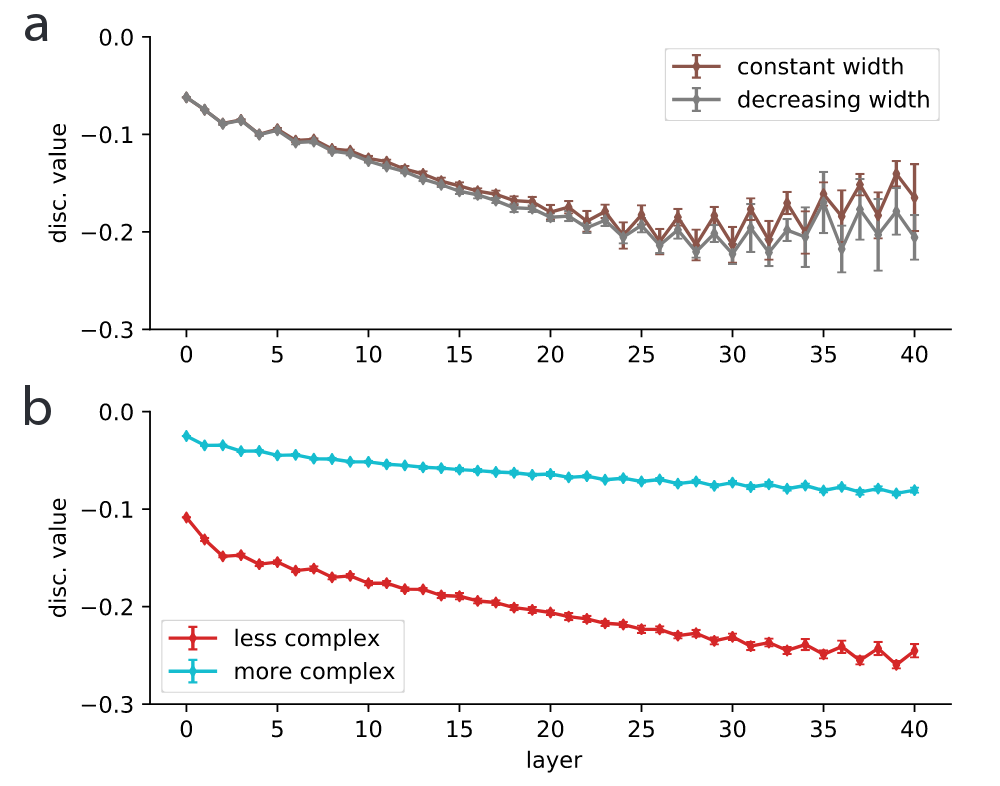
\includegraphics[width=9cm]{layers.png}
\end{center}
  \end{frame}

\begin{frame}{Results - reconstruction on MNIST}
  \vskip 1cm
  They reconstructed the images from different layers by taking the encoding, sparsifying it using $k$-winner takes all and then running the netowrk backwards to the input layer.
  \end{frame}

\begin{frame}{Results - reconstruction on MNIST}
\begin{center}
  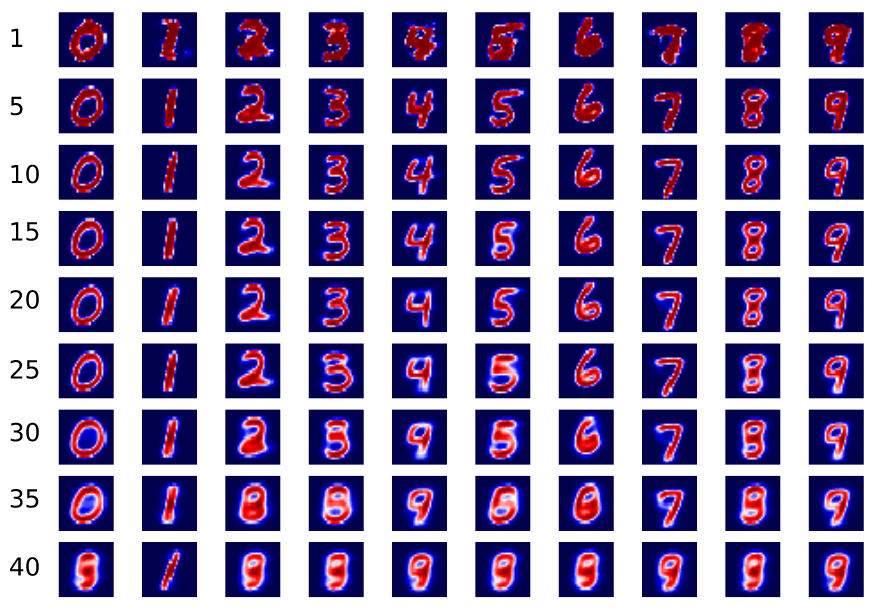
\includegraphics[width=9cm]{reconstruction.png}
\end{center}
  \end{frame}



\end{document}

